%Version 2.1 April 2023
% See section 11 of the User Manual for version history
%
%%%%%%%%%%%%%%%%%%%%%%%%%%%%%%%%%%%%%%%%%%%%%%%%%%%%%%%%%%%%%%%%%%%%%%
%%                                                                 %%
%% Please do not use \input{...} to include other tex files.       %%
%% Submit your LaTeX manuscript as one .tex document.              %%
%%                                                                 %%
%% All additional figures and files should be attached             %%
%% separately and not embedded in the \TeX\ document itself.       %%
%%                                                                 %%
%%%%%%%%%%%%%%%%%%%%%%%%%%%%%%%%%%%%%%%%%%%%%%%%%%%%%%%%%%%%%%%%%%%%%

%%\documentclass[referee,sn-basic]{sn-jnl}% referee option is meant for double line spacing

%%\documentclass[lineno,sn-basic]{sn-jnl}% Basic Springer Nature Reference Style/Chemistry Reference Style

%%\documentclass[pdflatex,sn-basic]{sn-jnl}% Basic Springer Nature Reference 
 
\documentclass[pdflatex, sn-nature]{sn-jnl}% Style for submissions to Nature Portfolio 

%%%% Standard Packages
\usepackage{graphicx}%
\usepackage{multirow}%
\usepackage{amsmath,amssymb,amsfonts}%
\usepackage{amsthm}%
\usepackage{mathrsfs}%
\usepackage[title]{appendix}%
\usepackage{xcolor}%
\usepackage{textcomp}%
\usepackage{manyfoot}%
\usepackage{booktabs}%
\usepackage{algorithm}%
\usepackage{algorithmicx}%
\usepackage{algpseudocode}%
\usepackage{listings}%
\usepackage{gensymb} %added by V. Van der Meersch
\usepackage{comment} %added by V. Van der Meersch
\usepackage{textcomp} %added by V. Van der Meersch
\newcommand{\textappr}{\raisebox{0.5ex}{\texttildelow}} %added by V. Van der Meersch
\usepackage{lineno} %added by V. Van der Meersch
\renewcommand\linenumberfont{\normalfont\tiny\sffamily\color{gray}} %added by V. Van der Meersch
\usepackage{changepage} %added by V. Van der Meersch


%%%%

%%%%%=============================================================================%%%%
%%%%  Remarks: This template is provided to aid authors with the preparation
%%%%  of original research articles intended for submission to journals published 
%%%%  by Springer Nature. The guidance has been prepared in partnership with 
%%%%  production teams to conform to Springer Nature technical requirements. 
%%%%  Editorial and presentation requirements differ among journal portfolios and 
%%%%  research disciplines. You may find sections in this template are irrelevant 
%%%%  to your work and are empowered to omit any such section if allowed by the 
%%%%  journal you intend to submit to. The submission guidelines and policies 
%%%%  of the journal take precedence. A detailed User Manual is available in the 
%%%%  template package for technical guidance.
%%%%%=============================================================================%%%%

%\jyear{2021}%

\raggedbottom
\unnumbered% uncomment this for unnumbered level heads

\begin{document}

\title[Article Title]{
% Temporary titles: Improving forecasting with process-based modeling
Biological mechanisms are necessary to improve projections of species range shifts}

\author*[1]{\fnm{Victor} \sur{Van der Meersch}}\email{victor.vandermeersch@cefe.cnrs.fr}
\author[2]{\fnm{Edward} \sur{Armstrong}}
\author[1]{\fnm{Florent} \sur{Mouillot}}
\author[3]{\fnm{Anne} \sur{Duputié}}
\author[4]{\fnm{Hendrik} \sur{Davi}}
\author[5]{\fnm{Frédérik} \sur{Saltré}}
\author[1]{\fnm{Isabelle} \sur{Chuine}}

\affil[1]{\orgdiv{CEFE}, \orgname{Univ Montpellier, CNRS, EPHE, IRD}, \orgaddress{\city{Montpellier}, \country{France}}}
\affil[2]{\orgdiv{Dept. of Geosciences and Geography}, \orgname{University of Helsinki}, \orgaddress{\city{Helsinki}, \country{Finland}}}
\affil[3]{\orgdiv{UMR 8198-EEP-Evo-Eco-Paleo}, \orgname{Université de Lille, CNRS}, \orgaddress{\city{Lille}, \country{France}}}
\affil[4]{\orgdiv{URFM}, \orgname{INRAE}, \orgaddress{\city{Avignon}, \country{France}}}
\affil[5]{\orgdiv{Global Ecology}, \orgname{College of Science and Engineering, Flinders University}, \orgaddress{\city{Adelaide}, \country{Australia}}}

\abstract{The recent acceleration of global climate warming has created an urgent need for reliable species distribution forecasts, widely used by natural resource managers. Such forecasts, however, are produced using various modeling approaches with little information on which perform well given expected novel climatic conditions. Here, we hindcast the range shift of five forest tree species across Europe over the last 12,000 years to compare the performance of three types of species distribution models and identify the origin of their robustness. We show that the performance of correlative models (CSMDs) decreases \textappr2 times faster than that of process-based models (PBMs) when climatic dissimilarity rises, and that PBM projections should be more reliable than CSDM ones at least up to 2060 according to scenario SSP245. These results reveal the major importance of describing biological mechanisms to ensure model robustness, and highlight a new avenue to improve model projections in the future.}    

\keywords{Ecological modelling, model transferability, species range shift,  tree species}

\maketitle

\newpage

% CUTE BABY: we need reliable projections of the distribution of species

% WEREWOLF: models perform less well under different conditions than those in which they were built/calibrated... and in addition, in the future, climatic conditions are expected to be very different
% And we don't know which model will be the most robust! :-( 

% SILVER BULLET: through this comparison in the Holocene, we highlight that it is necessary to model cause-and-effect relationships describing the abilities of species to survive/grow/reproduce in various env conditions
% and that inverse calibration using large-scale data may serve as an important step to facilitate the use of process-based models in a very near future :-) :-) :-) yippee!

\linenumbers
\section{Main}

Modelling is key to understand and forecast how climate change will impact ecosystems and biogeochemical cycles. Credible model projections are critical for natural resource managers, decision makers and stakeholders to make informed decisions. To meet the demand for reliable projections of ecosystems and biodiversity dynamics, thorough evaluations of ecological model performances should be a major focus \cite{Dawson2011, Mouquet2015, Pacifici2015}. 

One approach to evaluate model reliability is to compare their predictions to observations from previous time periods, i.e. hindcasting. Hindcasting can inform whether models capture, implicitly or explicitly, the essential processes required to provide reliable projections in conditions significantly different from the present. By looking far in the past, paleo-archives have proven to offer a unique opportunity to both understand long-term climate and biodiversity dynamics \cite{Bartlein2011, Fordham2020} and test model robustness and transferability (i.e. model capacity to maintain its performance in changing conditions \cite{UribeRivera2023}) \cite{Braconnot2012, Maguire2015}.  

However, thus far, models prediction of past species distribution and biospheric components have rarely been consistent with paleoclimate reconstructions and fossil records \cite{Veloz2012, Pearman2008, Roberts2012, Foley2013, Maguire2016} . Interpreting model projections in climatic conditions that differ significantly from the present, such as future no-analogue climatic conditions \cite{Williams2007}, thus raises questions. The guarantee that ecological model forecasts for the 21\textsuperscript{st} century will be reliable is therefore small \cite{Fitzpatrick2018}. 

While exact matches to expected 21\textsuperscript{st}-century climatic conditions do not exist in historical records \cite{Burke2018}, the dissimilarity between 20\textsuperscript{th} and 21\textsuperscript{st} century median climatic conditions (\hyperref[methods]{Methods}) falls within the range of dissimilarity encountered since the beginning of the Holocene (12 kyr BP, BP = Before Present (1950), \hyperref[climatic_dissimilarity]{Fig. 1}). This period takes place after the Last Glacial Maximum (26.5-19 kyr BP \cite{Clark2009}) and began with an abrupt climate warming followed by a long, almost uninterrupted, period of climatic stability until recent anthropogenic warming (Extended Data Fig. 1). The fossil pollen data accumulated over these last millennia provides us with an unique extended timeframe to test the reliability of ecological models, in particular those seeking to predict species distribution changes. %emw25Feb - this paragraph is great. 

\begin{figure}[ht]
\centering
\hspace*{-0.6in}
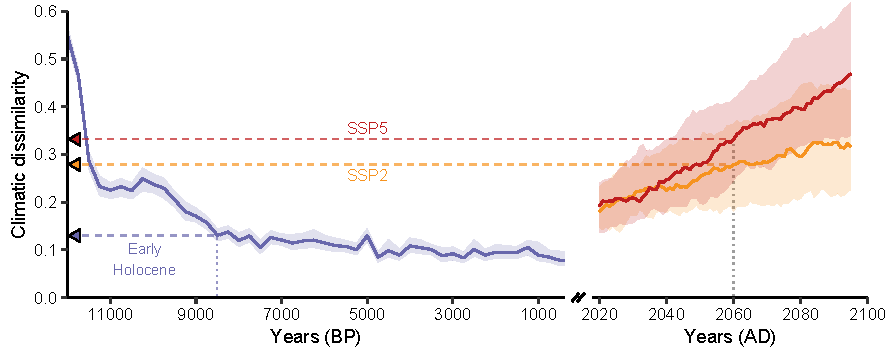
\includegraphics[scale=1]{climatic_dissimilarity.pdf}
\begin{adjustwidth}{-0.5cm}{-0.5cm}
\caption{\textbf{Evolution of climatic dissimilarity during the Holocene (12k-500 yr BP) and the 21st century (2005-2100), relative to 1901-2000}. Climatic dissimilarity is computed as 1-Sørensen similarity between bootstrapped climatic hypervolumes. Lines represent median dissimilarity, shaded areas represent 90\% confidence intervals. Blue corresponds to paleoclimate based on HadCM3B model. Yellow and red correspond to future climatic conditions according to SSP245 and SSP585 scenarios respectively, predicted by 34 global climate models of NEX-GDDP-CMIP6. The blue triangle on y-axis indicates the level of climatic dissimilarity 8500 years ago, at the limit between the Early and Late-Middle Holocene. Yellow and red triangles indicate the expected level of climatic dissimilarity in 2060 for SSP245 and SSP585 scenarios. Note that the x-axis scale is different between past and future panels.}\label{climatic_dissimilarity}
\end{adjustwidth}
\end{figure} %emw25Feb -- climatologists I know will want to know what you mean by 'climate model' ... if you have a short section in the supp where you define what you mean and list out the models -- and then reference that part of the supp here and in main text -- it might save you from cranky reviewers. 

Species distribution models (SDM) are powerful tools to predict species geographical distribution as a function of environmental data (e.g., mean annual temperature and annual total precipitation). Most studies have focused on correlative models (CSDMs, also called environmental niche models), which infer statistical relationships between observations of species occurrences and environmental predictors \cite{Dormann2012}. Their high flexibility and low computational complexity make them by far the most widely used tool for deciding on species conservation plans and policy regimes (e.g. \cite{Hanewinkel2013}). However, under novel climatic conditions, new unobserved portions of a species’ climatic niche may appear, which are not captured by these correlative approaches. For example, when challenged with distant past climates, CSDM predictive performance appeared to drop significantly \cite{Maguire2016}, which questions their ability to provide reliable projections in the future \cite{Fitzpatrick2018}. 

Alternative approaches to CSDMs are process-based models (PBMs) that rely on explicit formulations of the mechanisms driving the distribution of a given species (e.g., physiological, ecological and/or demographic processes). They come from decades of experiments and observations, including extreme conditions in laboratory \cite{Seehausen2017}, and climate manipulations such as CO\textsubscript{2} enrichment \cite{Jiang2020} or rainfall exclusion \cite{Gavinet2019}. The reliability of PBMs depends on our level of understanding of how ecophysiological processes are affected by environmental conditions, and the availability of large amount of observations to calibrate their many parameters \cite{Evans2016}. Because these models are not based on statistical relationships between present-day species occurrences (presence/absence) and environmental variables, and instead describe explicit causal relationships between biological processes and environmental variables, they are assumed to provide more reliable predictions of species distribution changes in novel climatic conditions  \cite{Evans2012, Singer2016}. However, another possible reasons why PBM projections might be more reliable than CSDM ones in novel climatic conditions might also come from their calibration method. Instead of being calibrated using species presence/absence data like CSDMs, PBM parameters are either measured directly (e.g. specific leaf area, leaf frost hardiness), and sometimes inferred statistically when they cannot be measured directly, using data on specific functional traits measured in the field or in laboratory (e.g. parameters of bud dormancy break date models). 

Despite the growing interest for PBMs in predictive ecology \cite{Connolly2017, Urban2016, Pilowsky2022}, the common assumption that they should provide more reliable projections of future species range shifts has never been verified. Nor have the reasons underlying this assumption been articulated. Qualitative models comparison in future climatic conditions have shown that PBMs often make more conservative projections in future climates than CSDMs which predict larger changes \cite{Morin2009, Cheaib2012, Gritti2013} but they have not provided any confidence level in these results. Very few studies have actually gone beyond qualitative comparisons between CSDMs and PBMs and compared thoroughly their performance, for example using virtual species \cite{Zurell2016}, exotic species in native and newly colonized areas \cite{Higgins2020}, or in the recent past \cite{Fordham2018}. 
While PBMs have shown their usefulness for paleoecological studies \cite{Saltre2013, Ruosch2016, Schwoerer2014}, the extent to which they can provide more reliable predictions than CSDMs in different climatic conditions from the historical period remains unknown \cite{UribeRivera2023, Briscoe2019}. 

Here, we address this critical gap by using multiple CSDMs and PBMs to simulate paleodistributions of five emblematic tree species of Europe at a high temporal resolution since 12 kyr BP. We used daily paleoclimatic data at 0.25° spatial resolution, generated from HadCM3B-M2.1 coupled general circulation model simulations, which includes both inter-annual variability, and millennial scale variability for rapid Dansgaard–Oeschger events before 11 kyr BP \cite{Armstrong2019}. Species migration ability was also incorporated in the simulations to represent more thoroughly changes in species realized distribution and not just not just changes in the distribution of species' climatic niches, so that an accurate comparison could be made with the paleorecords.

We first assessed which modelling approach best predicts past species distributions, and second whether model performance was related to their hypotheses (relationships describing explicit biological mechanisms or not) or to their calibration methods (calibrated on species occurrence data or not). To do so, we compared three types of models: CSDMs, PBMs (hereafter called expert PBMs) and fitted PBMs calibrated in the same way as CSDMs (inverse calibration using species occurrence data and a novel type of algorithm, \hyperref[methods]{Methods} and \citep{VanderMeersch2023}). The comparison between CSDMs/fitted PBMs and expert PBMs allowed us to determine whether the differences in model performance arise from their calibration methods, whereas the comparison between CSDMs and expert/fitted PBMs allowed us to determine whether the differences in model performance arise from the model hypotheses. We assessed the performance of the models for a maximum level of climate dissimilarity possible, i.e. over the last 12,000 years,  which corresponds to the climate dissimilarity expected by the end of the century according to SSP245, and by the middle of the century according to SSP585 ({Fig. 1}).

\begin{figure}
\centering
\vspace*{-0.6in}
\hspace*{-0.35in}
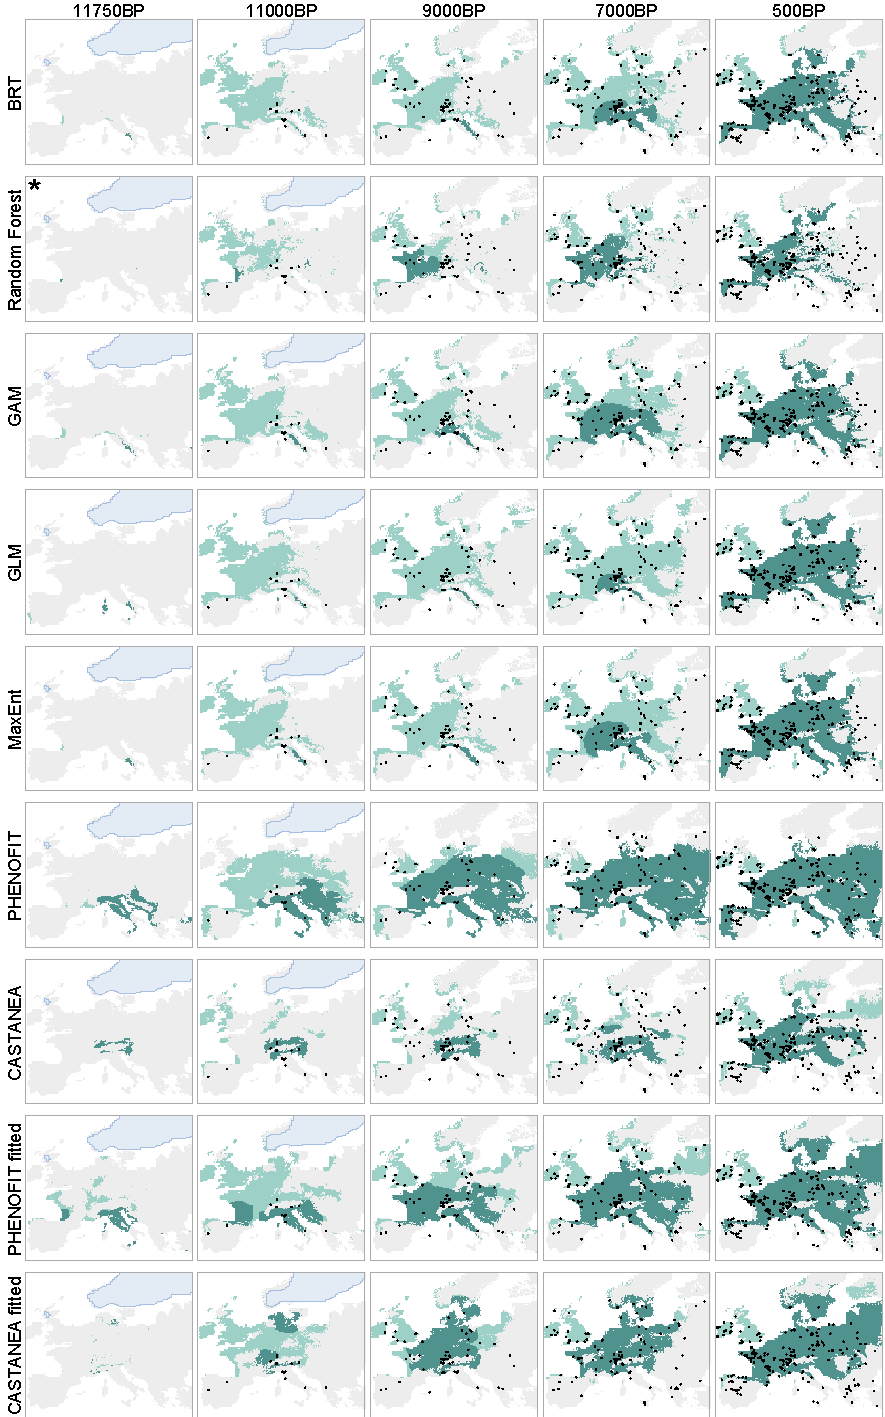
\includegraphics[scale=0.95]{quercus_deciduous_simulations-1.pdf}
\begin{adjustwidth}{-0.5cm}{-0.5cm}
\caption{\textbf{Example of paleosimulations obtained with the eight models used in this study for deciduous oaks.} The five first rows correspond to the five correlative models (boosted regression tree, down-sampled random forest, generalized additive model, generalized linear model with lasso regularization, MaxEnt). The four last rows correspond to two different versions (expert calibration and inverse calibration using occurrence data) of two process-based models (PHENOFIT and CASTANEA). Light green area is the modelled suitable area, dark green area is the colonized area (after migration). Light blue represents the ice sheet extent. Black dots are deciduous oak fossil pollen occurrences. The model for which migration started at 11.75 kyr BP rather than 12 kyr BP is marked with an asterisk. "BP" stands for "before present" (1950).}\label{quercus_migration}
\end{adjustwidth}
\end{figure}

\subsection{Mechanisms, not calibration method, convey model robustness and transferability }

As observed in previous long-term historical assessments, all models showed a decrease of their performance when moving further into the past, i.e. into more different climatic conditions than historical conditions (\hyperref[past_performance]{Fig. 3a}).
However PBMs showed smaller decrease in their predictive performance (slope of Beta regression, fitted PBMs: $-6.07$, 95\% CI $[-8.62, -3.55]$, expert PBMs: $-4.44$, 95\% CI $[-7.07, -1.77]$) than CSDMs ($-11.0$, 95\% CI $[-13.2, -8.91]$) (Fig. 3). PBMS also showed higher transferability in the most distant climatic conditions of the early Holocene than CSDMs (Fig. 3d). PBMs, either expert or fitted, are thus less affected by the increase in climate dissimilarity than CSDMs.  We further found that inverse calibration does not alter significantly PBMs performance and long-term transferability in most distant climate (Fig. 3).  These results suggest that models robustness and transferability are conveyed by the biological mechanisms they can describe rather than the methods of calibration.

In the near past (Late-Middle Holocene, $<$ 8.2 kyr BP), CSDMs were not significantly better at predicting tree distribution than any PBMs (pairwise Conover-Iman tests: \emph{vs.} expert PBMs \emph{t}-statistic $=1.68$/\emph{P} $=0.128$, \emph{vs.} fitted PBMs \emph{t}-statistic $=-1.55$/\emph{P} $=0.112$, \hyperref[past_performance]{Fig. 3b}), despite their closer fit to current species distributions (Extended Data Fig. 8). In the distant past (Early Holocene $>$ 8.2 kyr BP), CSDMs performed worse than both expert and fitted PBMs (pairwise Conover-Iman tests: respectively \emph{t}-statistic $=-4.80$/\emph{P} $<0.0001$ and \emph{t}-statistic $=-5.07$/\emph{P} $<0.0001$, \hyperref[past_performance]{Fig. 3b}). 

Both types of PBMs, fitted and expert, were more performant than CSDMs to predict species recolonisation dynamics in the Early Holocene (\textappr11.5-8.5 kyr BP)  because they predicted more accurately refugia locations at -12 kyr BP which were the starting points for the migration cellular automaton model (\hyperref[quercus_migration]{Fig. 2} and \hyperref[methods]{Methods}). This period  corresponds to a global deglaciation which lasted for a few centuries and occurred after the cooling of the Younger Dryas interval  (\textappr13-11.5 kyr BP, Extended Data Fig. 1). This rapid warming episode explains the strong decrease of climate dissimilarity relative to present between 12 kyr BP and 11.5 kyr BP (\hyperref[climatic_dissimilarity]{Fig. 1}). Simulating migration allowed us to take into account the differences between the models during this 500-year interval, in the most challenging conditions when the climate dissimilarity was the strongest and the closest to what we will experience by the end of the century. Since the migration model is identical across all simulations, differences of performance between models across the Holocene very much depend on their ability to predict the potential refugia of the species during the Early Holocene. For example, some models were not able to predict evergreen \emph{Quercus} refugia in Southern Spain, and thus missed an important migration route and failed predicting their presence in vast areas in the Late Holocene (Extended Data Fig. 6). As PBMs, either fitted or expert, describe the response of ecophysiological processes to a wide range of environmental conditions, they may provide a better estimation of the conditions where species could have survived 12000 years ago, in more dissimilar climates. If we had not considered the 12-11.5 kyr BP period of high climatic dissimilarity (i.e. without simulating migration from refugia), we would have missed the opportunity to take into account model projections within the same dissimilarity level to what we expect between 2050 and 2100 (\hyperref[climatic_dissimilarity]{Fig. 1}), and CSDMs and PBMs' abilities to predict fossil pollen occurrence would have been similar (Extended Data Fig. 10cd), with an average Sørensen index decrease of $-0.205\pm0.0224$ (paired Wilcoxon-test: \emph{P} $<0.0001$) between Late-Middle Holocene and Early Holocene.

Models performances were not stable across species, and exhibited both similarities and differences across time (Extended Data Fig. 9). More specifically, models exhibited the same overall performance decrease against \emph{Fagus} pollen records, whereas CSDM performance decline was substantially faster than expert and fitted PBMs for deciduous \emph{Quercus}. All models show low predictive power regarding evergreen \emph{Quercus} distribution even in the Late Holocene compared to other species, especially CSDMs which failed to predict its presence along the Atlantic coast (Extended Data Fig. 6). Fitted PBMs, however, showed the lowest variability of performance across species (\hyperref[past_performance]{Fig. 3c}).

A potential limitation of our approach is that we cannot account for very rare and really long-distance dispersion events, as well as the influence of humans. For example all models failed to predict deciduous \emph{Quercus} in the British Isles before the Early Holocene sea level rise and the opening of the Strait of Dover (\hyperref[quercus_migration]{Fig. 2} and \cite{Smith2011}), even though the land-sea mask changed throughout the simulations. However, we cannot assert whether this is due to misrepresented very long-distance dispersion events of seeds, e.g. by humans or jays, across major dispersal barrier, or a misprediction by all models of more northern refugia.

\begin{figure}[ht]
\centering
\hspace*{-0.8in}
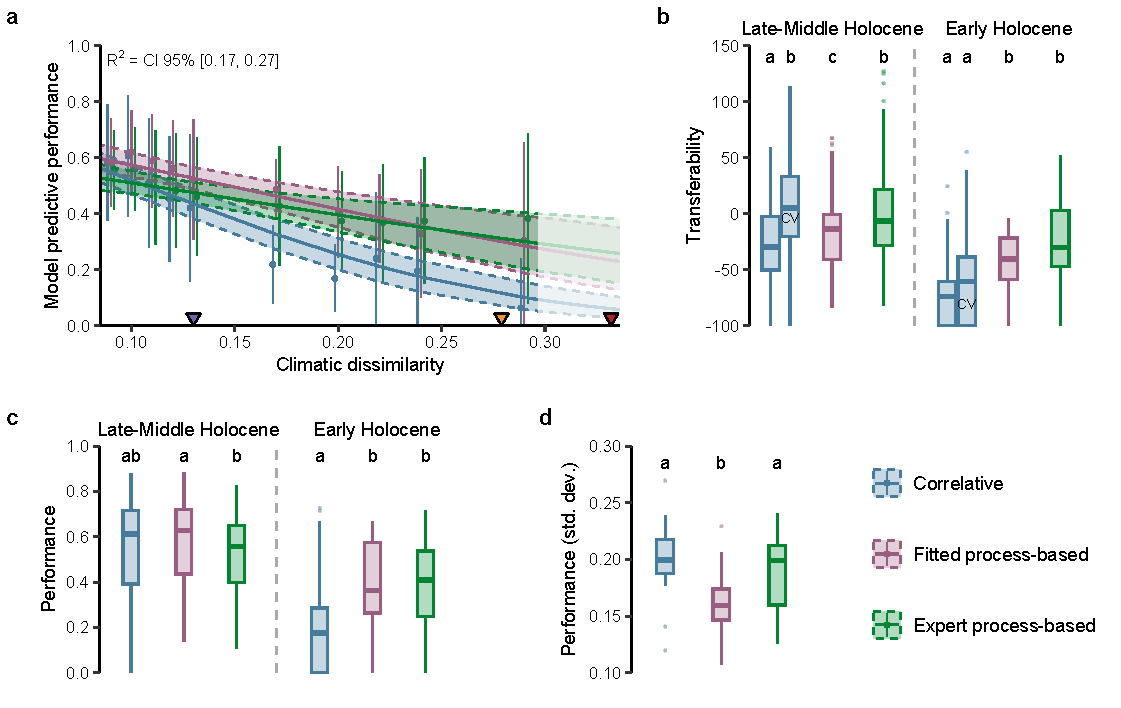
\includegraphics[scale=0.9]{past_performance.pdf}
%emw13Jan -- can you add the SSP labels to triangles on Fig a?
\begin{adjustwidth}{-0.5cm}{-0.5cm}
\caption{\textbf{Performance of correlative models, fitted process-based models (inverse calibration using occurrence data) and expert process-based models (classical calibration) against Holocene paleoecogical evidence (fossil pollen) for 4 tree genera (\emph{Abies}, \emph{Fagus}, \emph{Quercus} deciduous and \emph{Quercus} evergreen).} \textbf{(a)} Bayesian beta regression of model predictive performance (Sørensen index) against climatic dissimilarity relative to 1901-2000 (1-Sørensen similarity between climatic hypervolumes). Shaded areas represent 2.5\% and 97.5\% quantiles of the posterior predictive distribution. Points represent the average model performance (and lines the standard deviation) grouped by similar level of climatic dissimilarity. Blue triangle on x-axis indicates the limit between Early Holocene ($>$ 8.2 kyr BP) and Late-Middle Holocene ($<$ 8.2 kyr BP). Yellow and red triangles indicate the expected level of climatic dissimilarity in 2060 for SSP245 and SSP585 scenarios. Legend on the right: top row represents drivers of modelled distributions (correlations/mechanisms), bottom row represents calibration method (species distributions/measurements). Panels \textbf{(b)} and \textbf{(c)} show the difference in performance (Sørensen index) and variability in performance (standard deviation of Sørensen index) across models. Panel \textbf{(d)} shows the transferability of the models (relative change in model performance between distant past periods and historical period). A negative transferability means that model performance is lower in the distant past periods than in the historical period. CSDM predictive errors in the historical period was assessed by two different methods: (i) against the same data used for calibration (leading to an overestimation of historical model performance -- but more comparable to fitted PBM estimates), (ii) using an environmental block cross-validation, noted as "CV" (leading to a better estimation of true model errors in the historical period, and thus a higher transferability -- but less comparable to fitted PBMs for which cross-validation would have been too computationally expensive). The grouping letters represent the multiple comparisons with pairwise Conover-Iman tests. }\label{past_performance}
\end{adjustwidth}
\end{figure}

\subsection{Scaling-up process-based models}

Our results show that model transferability and robustness is rather conveyed by the mechanisms represented in the models than by their method of calibration. Therefore, in addition to allowing separate investigation of the effects of environmental stresses on tree survival, growth, and reproduction, biological mechanisms represented in PBMs are critical to ensure higher model robustness in more novel climatic conditions. This is an important and new result which both argues for a wider use of PBMs to provide forecasts of biodiversity and ecosystems distributions in the future and opens a new avenue  to reach this goal by using inverse modelling technics to calibrate them.

Fitted PBMs bring together the strengths from both CSDMs and expert PBMs approaches by describing causal relationships between environmental conditions and species performance (i.e. from process-based approaches) and precise estimates of parameter values (from correlative approaches). Indeed, inverse calibration improved process-based projections in Middle-Late Holocene, when climate conditions were not  drastically different from present: performances of fitted PBMs was higher than those of expert PBMs (\emph{t}-statistic $=2.70$/\emph{P} $=0.020$, \hyperref[past_performance]{Fig. 3b}). These differences between expert and fitted PBMs in the Middle-Late Holocene pinpoint some issues in expert parameterization that requires to combine various methods to cope with both the scarcity of data for each ecophysiological process modelled and sometimes non-measurable parameters (e.g. \citep{DeCaceres2023}).  Some parameters in these relations can be measured directly, and exhibit little variability across a species range (e.g. water potential leading to 50\% of vessels embolism). However, the measurement of parameters in controlled conditions does not necessarily guarantee their external validity \emph{in natura} \cite{Asse2020} where much more factors, not represented in laboratory conditions, can also affect the process modelled (but see \cite{Satake2013}). Other parameters are either highly variable because of local adaptation over long period,  difficult-to-measure or so far unmeasurable (e.g. bud dormancy). Therefore, expert PBMs can suffer from uncertainties entailed in the measurements of some of their parameters, and from spurious data specific to few locations which do not represent sufficiently well all the conditions the species can experience all over its range. For all these reasons, inverse calibration can provide a valuable opportunity to estimate the values of PBM parameters especially difficult to estimate otherwise \cite{Evans2016, Hartig2014}. However, inverse calibration using only occurrence data could lead to a misrepresentation of true processes \cite{VanderMeersch2023}, and is only a first step towards a better calibration of PBMs. 

\subsection{Can model performance in the past give a hint of their performance in the future?}
%emwFeb25 -- I really liked the title, 'Can model performance in the past give a hint of their performance in the future?' But then the whole section was just basically caveats without emphasizing what you found or mean. So it really answered the questions with a DOWN note and emphasized problems. Instead, I would suggest opening this section with more an overview that says 'our hind casting results suggest XYZ for the future' and then rephrase some of the caveats as critical areas for new research or more positive. For example, instead of saying 'Despite different future projections among global climate models (Extended Data Fig. 2), the rate of anthropogenic climate change and the increased probability of occurrence of novel climates ([13] and Fig. 1) are challenging...' You could say more 'our approaches are built on the current climate projections (some caveats on these), but can be updated as improved projections are available.' And for the pollen data: We found the starting point of the simulations at 12 kyr BP played a major role in the evaluation of models performance across the Holocene (Extended Data Fig. XX), suggesting the importance of starting conditions for these models. [Explain this then in terms of what it means for projections -- starting conditions TODAY .. which you have, then discuss issues with pollen record affecting model results.]
%emw13Jan -- below is great!
Our hindcasting results suggest that predictions of PBMs, either fitted or expert, should be more reliable at least up to 2060 according to the scenario SSP245 (\hyperref[past_performance]{Fig. 3a}) and 2050 according to SSP585. The rate of anthropogenic climate change and the increased probability of occurrence of novel climates (\cite{Williams2007} and \hyperref[climatic_dissimilarity]{Fig. 1}) are challenging the reliability of both CSDMs and PBMs especially when they are intended to be used in more complex models such as biosphere-atmosphere models and by natural resource managers and policy makers to guide management plans and policies. Acknowledging these uncertainties is as important as making the forecasts themselves \cite{Beale2012} and contributes to the public trust in scientists \cite{Berkhout2010}. Our approach is built on the current climate projections, which varies among global climate models (Extended Data Fig. 2b), but can be updated as improved projections are available. 

The recent efforts to gather fossil pollen data and make them openly available \cite{Williams2018} allow us to objectively assess model performance in very different conditions from those used for their calibration. From 11.5 kyr BP onwards, climate dissimilarity varies between 0.29 and 0.08, a level equivalent to what we might experience in the second quarter of the 21st century (\hyperref[climatic_dissimilarity]{Fig. 1}). Model consistency with past observations does not demonstrate that the model will be valid in the future \cite{Oreskes1994}, but we make here a critical step towards enhancing our understanding of model transferability. As more and more pollen data becomes available, we could cover a wider range of conditions, prior 11.5 kyr BP. Incorporating migration has nevertheless enabled us to observe that the accuracy of the starting point of the simulations at 12 kyr BP, when climatic dissimilarity was at its highest, played a major role in assessing the performance of the models throughout the Holocene. Our simulations have transitioned from these very different initial climatic conditions to a climate more analogous to historical state. The uncertainties on the initial conditions had thus a significant influence on the simulation outcomes. In the future, on the contrary, initial uncertainties will be much lower as models will start from the known distributions of species. However, uncertainties will rise as simulations proceed towards increasingly dissimilar climatic conditions, all the more since these latter will shift outside the range experienced in the past (Extended Data Fig. 3).

While it is still a challenge to make a solid quantification of models projections uncertainty, our results open new avenues for model evaluation improvement. The discrepancies between model performances we observed highlights the importance of considering various modelling methods to capture the full range of uncertainties associated with future projections. It implies that we should not rely solely on the model's own prediction dispersion to estimate projection uncertainties, nor on very similar modelling approaches, especially when climate dissimilarity sharply increases. Moreover, models will have to consider that tree colonization dynamics will likely be very different in the future: it will not only occur from a few refugia but from wider continuous ranges, and direct anthropogenic factors, such as sylvicultural practices and assisted species migration, will also shape the composition of forests \cite{Aitken2016}.

% \subsection{Conclusion}
% CSDMs can teach us process-based model-building strategies that allow for the propagation of errors, and allow to separate uncertainty sources within model (imprecise parameters, input data, ...) ?
% Hybrid approach: "\emph{Interest to balance biological realism and flexibility in model building with limited knowledge}" (IPBES, chapter 4) => citation à rajouter peut-être qq part
% idea in Evans 2012: forecast need to be realistic and need to be reliable in novel conditions \cite{Evans2012} (two conditions) + ! 
To conclude, the unique multi-model comparison across the Holocene we provide here suggests that our understanding of biological mechanisms embedded into process-based models represent a real advantage as compared to empirical relations used in CSDMs to increase projections reliability in the upcoming decades. However, data availability places limits on how these models can be parameterized, and could explain the difficulty to use them more widely for global impact studies. Fitted PBMs may overcome this problem by using more data at a larger geographical scale, while keeping the predictive strength of causal relationships. Given ongoing improvements in computational methods and newly available measurements at global scale (e.g. forest structure and growth with remote sensing and LiDAR data), there is an avenue for an extensive calibration and use of process-based models to provide more reliable projections in the next decades.

\section{Methods}\label{methods}

\subsection{Correlative and process-based models}\label{models}

We used two process-based models which differ by their underlying hypothesis and complexity. 
PHENOFIT simulates the fitness of an average adult tree \cite{Chuine2001}. It estimates fitness components (survival and reproductive success) by simulating the precise phenology (dates of leaf unfolding, flowering, fruit maturation, leaf senescence) and damages caused by abiotic stress (frost, drought) which effects depend on their occurrence relatively to the development stages of the different organs. It has been validated for several North American and European species \cite{Morin2007, Saltre2013, Duputie2015, Gauzere2020}. The model has \textappr30 parameters. 
CASTANEA simulates carbon and water cycles of an average adult tree by simulating many processes such as photosynthesis, stomatal opening, maintenance and growth respiration, transpiration and carbon allocation  \cite{Dufrene2005}. It has been used to predict carbon and water budgets of several European species \cite{Davi2006, Delpierre2012, Davi2017}. 
The model has \textappr80 parameters. 
Both models require daily meteorological variables and soil characteristics. 
%emw13Jan -- The below needs to be clearer for readers in the main text I think. 
Two versions of both models were employed: one was calibrated with expert knowledge and statistical inference using observations and measurements of the processes modelled (version called \emph{expert}), and a second one was  entirely calibrated using species distribution data (version called \emph{fitted}, \cite{VanderMeersch2023}) like correlative models. For the latter, we used the optimization algorithm CMA-ES \cite{Hansen2001} as described in \cite{VanderMeersch2023}, and retained the best calibrations in terms of AUC.
  
We selected correlative models based on the thorough model comparison made by Valavi et al. \cite{Valavi2022}. Among the most performant models, we selected five well-established models: GLM with lasso regularization, GAM, BRT, MaxEnt and down-sampled Random Forest. Some of these models are known to struggle when applied to extrapolation domains, but are nevertheless widely used by ecologists to provide projections of species distribution change in future climatic conditions.
We chose four uncorrelated climate predictors related to ecological processes to calibrate these models: minimum temperature of the coldest month (representing frost tolerance), total precipitation (representing available water), GDD5 (growing degree days  \textgreater5°C) between April and September (representing available thermal energy for vegetation growth and fruit maturation), water balance between June and July (precipitation$-$evapotranspiration, representing summer drought tolerance). We also included two soil covariates (pH and Water Holding Capacity).
  
While by construction correlative models directly output species habitat suitability, we used fitness predicted by the model PHENOFIT and net primary production predicted by the model CASTANEA as a proxy of species habitat suitability as they have already been used to predict species presence in previous studies \cite{Morin2009, Cheaib2012, Saltre2013}. 
CSDMs and inverse-calibrated PBMs were calibrated for five species (\textit{Fagus sylvatica} L., \textit{Abies alba} Mill., \textit{Quercus robur} L., \textit{Quercus petraea}  (Matt.) Liebl. and \textit{Quercus ilex} L.) using historical climate (1970-2000) extracted from ERA5-Land hourly dataset \cite{MunozSabater2021}, soil data from EU-SoilHydroGrids \cite{Toth2017} and SoilGrids \cite{Hengl2017} databases and species presence data from the dataset assembled in \cite{VanderMeersch2023}, mostly based on EU-Forest inventory data \cite{Mauri2017}. To calibrate the CSDMs, we additionally sampled 50,000 background points, which should properly represent the variation in the environmental conditions across the study area \cite{Valavi2022}. For each CSDM and each species, we run a fivefold environmental cross-validation to estimate model performance in novel extrapolation conditions (Extended Data Fig. 8 and \cite{Roberts2017}). We then used all the available training data to calibrate the models for the hindcasting in order to favour final prediction quality \cite{Roberts2017}. We could not run the same cross-validation method for fitted process-based models because it would have been too computationally expensive. 

Model simulations over the Holocene were run for 30-year periods every 250 years, for the five above mentioned species. Model outputs were averaged over each 30-year period. Note that soil conditions (needed both for correlative and process-based models) were held constant throughout the simulations, and were bilinearly interpolated from closest coastal cells where data was missing (because of different land-sea masks between present and past). Note also that for CASTANEA model, species-specific thresholds of net primary production determining the presence or absence of the species were computed with the CO$_2$ level at the beginning of the Holocene (\textappr240ppm).

\subsection{Late Quaternary climate and vegetation}\label{paleodata}
%emw13Jan -- are there multiple initial conditions (members)? Not critical, I am just wondering. 
We used a monthly paleoclimate simulation dataset \cite{Armstrong2019} generated with the HadCM3B-M2.1 coupled general circulation model, starting from 18 kyr BP at 0.5\degree~spatial resolution for Europe (Extended Data Fig. 1). It includes both inter-annual variability, and millennial scale variability for rapid Dansgaard–Oeschger events before 11 kyr BP. For this work, several variables were specifically produced: mean temperature, average minimum and maximum daily temperatures, precipitation, number of rainy days, cloudiness, and wind speed. We further downscaled temperature and precipitation monthly data to 0.25\degree~resolution, by applying an elevation correction of coarse-scale variables towards the ICE-6G-C elevation level at high resolution \cite{Peltier2015}.  
We then generated daily data for temperatures, precipitation, cloud cover and wind speed from  the monthly data with the weather generator GWGEN \cite{Sommer2017}, for 30-year periods every 250 years. We also simulated daily extra-terrestrial solar radiation with the same orbital forcing conditions used in HadCM3B-M2.1 \cite{Armstrong2019} and then computed daily global radiation taking into account previously generated daily cloud-cover data as implemented in LPJ-LMfire global model \cite{Pfeiffer2013}. Finally, we computed daily potential evapotranspiration following the standard FAO Penman-Monteith method \cite{Allen1998}.  

Fossil pollen records were extracted from the LegacyPollen dataset \cite{Herzschuh2022}. This dataset is mainly based on the Neotoma database \cite{Williams2018}, and provides samples with standardized chronologies and age uncertainties. We removed sites that had marine depositional environments \cite{Maguire2016}, and only kept samples with more than 200 pollen grain counts and age uncertainty of less than 500 years.
Pollen relative abundances were aggregated to consecutive 500-year intervals. If multiple samples from the same site belonged to the same period, we averaged their pollen abundances, weighting by their age uncertainty and temporal distance from the center of the period. Relative pollen abundances were converted to presence/absence using thresholds based on biome reconstructions \cite{Williams1998}: 1\% for \emph{Fagus} and \emph{Abies}, and 2.5\% for \emph{Quercus}. If several sites fell within the same grid cell (0.25\degree), we considered the species as present if there was at least one site where the species could be considered as present. \textit{Fagus} pollen data were used to assess the presence of \textit{Fagus sylvativa} L., sole species of the genus present in Europe. \textit{Abies} pollen data were used to assess the presence of \textit{Abies alba} Mill., most abundant and widespread fir species present in Europe. When possible, deciduous and evergreen \textit{Quercus} pollen were distinguished based on Neotoma data. Some \textit{Quercus} pollen remain undetermined beyond the generic level, either because discrimination between evergreen and deciduous oak pollen was impossible or because authors were not specific. They were assigned to two categories, based on the evergreen natural range as defined by Atlas Flora Europeae \cite{AFE2005} and EuroVegMap \cite{EVM2003}: pollen outside range were considered as deciduous only occurrences, whereas pollen inside range were considered as both evergreen and deciduous occurrences. Deciduous \textit{Quercus} pollen data were used to assess the presence of \textit{Quercus} \textit{petraea}  (Matt.) Liebl., and \textit{Quercus robur} L., the two most abundant and widespread deciduous oak species in Europe. Evergreen \textit{Quercus} pollen data were used to assess the presence of \textit{Quercus ilex} L., the most abundant and widespread evergreen oak species in Europe.

\subsection{Tree migration}\label{migration}

Models used in this study predict species potential distribution based solely on climatic and soil conditions. To compare model predictions to pollen paleorecords, species migration needs to be simulated as well, as it can be the primary factor limiting species distribution before climatic conditions, especially when climatic conditions are changing rapidly as it was the case during the Dansgaard–Oeschger events \cite{Svenning2004, Saltre2013}.  \\
To implement migration in the simulations, we run a  cellular automaton \cite{Engler2012} which has proven to be as accurate as more complex approaches \cite{Zurell2016}. We modified the initial version of this dispersal model in order to use both short- and long-distance dispersal kernels. We used species-specific fat-tailed kernels \cite{Zani2022} at a 500 m resolution, and assumed that trees can disperse once a year (Extended Data Fig. 7a). Model outputs were assigned to two classes using specific optimal thresholds maximizing model performance (TSS) in the historical climate (Extended Data Fig. 8): (i) cells where the model output was under the specific threshold were assigned a zero suitability (species cannot survive), and (ii) cells where the  model output was above the threshold, the suitability was rescaled between 0 and 1 (species can migrate). We considered the deciduous \emph{Quercus} suitability as the maximum suitability between \emph{Q. robur} and \emph{Q. petraea}. Migration simulations started from 12 kyr BP (or 11.75 kyr BP when a model simulates no presence at 12 kyr BP). Note that starting at 11.75 kyr BP or 12 kyr BP does not change our results (Extended Data Fig. 10e-h), and that we could not start earlier (e.g. \textappr15 kyr BP) as most models predict no presence at all around 12.5 kyr BP. We also checked that dispersal process stochasticity at 500m resolution (Extended Data Fig. 7a) had no significant effect on the model's performance at the scale of Europe, by simulating deciduous \emph{Quercus} migration 10 times for each of the 8 models (Extended Data Fig. 7b). 

\subsection{Models' performance}\label{skill}

We used the Sørensen's similarity index to measure the hindcast performance of the models, based on the confusion matrix. This discrimination measure has been shown to provide adequate estimations of model discrimination capacity,  not biased by species prevalence or an inflated number of true negative predictions \cite{Leroy2018}. This feature is important when working with fossil pollen data, for which the number of species absence can be much higher than the number of species presence. Note that we obtained similar results when using TSS as the performance metric (Extended Data Fig. 10b). We compared the area potentially occupied (not taking migration into account) and occupied (taking migration into account) by the species to the presence/absence data extracted from the LegacyPollen dataset every 500-year interval. Kruskal-Wallis tests followed by multiple pairwise post-hoc Conover-Iman tests (using Benjamini-Yekutieli adjustment, as implemented in the R package \emph{conover.test}) were computed to assess stochastic dominance among model performance and transferability (\hyperref[past_performance]{Fig. 3b-d}).

In order to quantify the climatic differences between  historical climate (1901-2000, based on the CRU TS v. 4.07 gridded dataset \citep{Harris2020}) and Holocene climate (hindcasting conditions), we computed the \emph{climatic dissimilarity} as the Sørensen dissimilarity between climatic hypervolumes (a metric of overlap in multidimensional space). We first generated for each period (500-year intervals from -12 kyr BP to 500 BP and 1901-2000) a set of 20 bootstrapped hypervolumes, using R package \emph{hypervolume} \cite{Blonder2018}. Hypervolumes were computed with a Gaussian kernel density estimation method based upon the first three principal component axis from three-month means temperature and three-month sums of precipitation. We then computed overlap statistics (mean and standard deviation of Sørensen index) between the bootstrapped hypervolumes of each time points of the Holocene and the bootstrapped hypervolumes of the historical period (i.e. 20x20 overlaps). As a comparison, we also computed the climate novelty based on Mahalanobis distance (\citep{Burke2019} and Extended Data Fig. 2). 
We also computed these metrics for future conditions in order to compare the dissimilarity of future climate to that of  the Holocene climate, both relative to 20th century climate. To assess future conditions, we used all the global climate models from NEX-GDDP-CMIP6 dataset \citep{Thrasher2022} (except HadGEM3-GC31-MM, not available for SSP245) and 2 scenarios (SSP245 and SSP585). To make the comparison, both paleoclimate and future climate data were uniformized with the CRU dataset to maximize comparability between paleoclimate and future climates. The difference (for three-month temperature average) and the ratio (for three-month precipitation sum) between the observations (from 1901 to 2000) and simulations (1901-1950 for HadCM3B, 1951-2000 for CMIP6 projections) were calculated and applied to the whole modelled time period, assuming that the bias was constant. 

Finally, we estimated the effects of past climate novelty (Sørensen's climatic dissimilarity) on model performance (Sørensen index) with a Bayesian ordered beta regression, considering the different types of models (correlative, fitted process-based and expert process-based), using the R package \emph{ordbetareg} \cite{Kubinec2023} and RStan \cite{SDT2023}. Compared to a  standard beta regression model, this model allows for observations at the bounds (i.e. Sørensen index = 0 or = 1). We took into account the standard deviation of Sørensen's climatic dissimilarity (computed with sets of bootstrapped hypervolumes, see above) as a predictor measurement error.

\backmatter

\section*{Data and code availability}

Simulation outputs, together with the code to reproduce the analysis and figures in this study, are available on GitHub at \url{https://github.com/vvandermeersch/past_robustness}.

\section*{Acknowledgments}

The authors are deeply grateful for many helpful comments from Elizabeth M. Wolkovich, which have greatly enriched this manuscript. They would also like to thank Christophe Randin for his valuable input throughout the course of this research, and Jed O. Kaplan for making GWGEN and LPJ-LMfire codes openly available.\\
They acknowledge the support and computing resources of GenOuest and TGCC-CEA.
Future climate scenarios used were from the NEX-GDDP-CMIP6 dataset, prepared by the Climate Analytics Group and NASA Ames Research Center using the NASA Earth Exchange and distributed by the NASA Center for Climate Simulation (NCCS). They acknowledge the World Climate Research Programme, which, through its Working Group on Coupled Modeling, coordinated and promoted CMIP6.\\
V.V. was supported by a PhD Fellowship from the GAIA doctoral school of the University of Montpellier, France.

\section*{Ethics declarations}

The authors declare no competing interests.

%%===========================================================================================%%
%% If you are submitting to one of the Nature Portfolio journals, using the eJP submission   %%
%% system, please include the references within the manuscript file itself. You may do this  %%
%% by copying the reference list from your .bbl file, paste it into the main manuscript .tex %%
%% file, and delete the associated \verb+\bibliography+ commands.                            %%
%%===========================================================================================%%

\bibliography{robustness_bibliography}% common bib file
%% if required, the content of .bbl file can be included here once bbl is generated
%%\input sn-article.bbl


%%Online only Methods should be presented in a separate section after the end of the main text
%% and reference list




\end{document}
